\documentclass[
  11pt,
  letterpaper,
   addpoints,
  answers
  ]{exam}

% Carga el preámbulo localizado en la carpeta superior
\NeedsTeXFormat{LaTeX2e}[2023/04/30]

% Provide the name of your page, the date it was last updated, and a comment about what it's used for
\ProvidesPackage{../exercise-preamble}[2023/04/30 Prof. Cassanelli custom LaTeX style]

% \usepackage{printlen}
% \uselengthunit{in}\printlength{\textwidth}

% PACKAGES
\usepackage[dvipsnames]{xcolor}

\usepackage{graphicx}
\graphicspath{{../figures}}
\usepackage{amsmath,amsthm,amssymb,mathtools,mathrsfs}
\usepackage{commath}
\usepackage{upgreek}
\usepackage{cancel}
\usepackage{enumerate}
\usepackage[font=small]{caption}
\usepackage[normalem]{ulem}
\usepackage{steinmetz}

\usepackage[left=1.5cm, right=1.5cm, top=1cm]{geometry}

% REFERENCES AND OTHERS
\usepackage{../aas_macros}
\usepackage{natbib}
\bibpunct{(}{)}{;}{a}{}{,}

\usepackage{tikz}
\usepackage{tikz-3dplot}
\usepackage{circuitikz}
\usepackage{pgfplots}
\pgfplotsset{compat=1.15}
\usepgfplotslibrary{smithchart}
\usetikzlibrary{
  decorations.pathmorphing,
  decorations.markings,
  calc,
  patterns,
  decorations,
  angles,
  quotes,
  ext.topaths.arcthrough,
  shapes
  }

\usepackage{siunitx}
\sisetup{
    range-phrase=\text{--},
    range-units=single,
    separate-uncertainty=true,
    print-unity-mantissa=false
    }
\DeclareSIUnit{\gauss}{G}
\DeclareSIUnit{\jansky}{Jy}

\newcommand{\iu}{\mathrm{i}\mkern1mu}
\newcommand{\ju}{\mathrm{j}\mkern1mu}
\newcommand{\euler}{\mathrm{e}}
\newcommand{\exponential}[1]{\mathrm{exp}\left[#1\right]}
\newcommand{\uvec}[1]{\widehat{\mathbf{#1}}}
\newcommand{\uvecs}[1]{\boldsymbol{\widehat{#1}}}
\newcommand{\bvec}[1]{\boldsymbol{\mathcal{#1}}}

\usepackage{hyperref}
\hypersetup{
    % bookmarks=true,
    unicode=true,
    pdftoolbar=true,
    pdfmenubar=true,
    pdffitwindow=false,
    pdfstartview={FitH},
    pdftitle={EL3103},
    pdfauthor={Tomas Cassanelli},
    pdfcreator={Tomas Cassanelli},
    pdfnewwindow=true,
    colorlinks=true,
    linkcolor=Violet,
    citecolor=Violet,
    urlcolor=Violet
    }

% Exam document class
\renewcommand{\figurename}{Figura}
\renewcommand{\tablename}{Cuadro}
\pagestyle{empty}

\usepackage[spanish]{cleveref}

\crefname{question}{\protect{pregunta}}{\protect{preguntas}}
\Crefname{question}{\protect{Pregunta}}{\protect{Preguntas}}
\creflabelformat{question}{#2{#1}#3}

\renewcommand{\solutiontitle}{\noindent\textbf{Solución:}\par\noindent}
\bracketedpoints
\pointname{~puntos}

\endinput

% Paquetes locales
\usepackage{float}
\usepackage{booktabs} % para \toprule, \midrule, \bottomrule
\usepackage{xcolor} % para colores
\usepackage{bm} % para negrita en símbolos matemáticos

% Macros locales
\newcommand{\Rel}{\mathfrak{R}} % símbolo para la reluctancia

\begin{document}

% Configuración del encabezado usando comandos de la clase exam
\pagestyle{headandfoot}
\extraheadheight{0.5in} % Baja el encabezado aumentando el espacio superior
\firstpageheader{\textit{Análisis de Sistemas Dinámicos y Estimación}}{}{EL3204-1}
\runningheader{\textit{Análisis de Sistemas Dinámicos y Estimación}}{}{EL3204}
\firstpagefooter{}{\thepage}{}
\runningfooter{}{\thepage}{}
\headrule % Línea debajo del encabezado

% Numeración de página
\pagenumbering{arabic}

% Portada
\begin{center}
    \vspace*{1cm}
    
    % Logo superior
    \includegraphics[width=0.5\textwidth]{../fcfm_die}
    
    \vspace{2cm}
    
    % Líneas decorativas superiores
    
\begin{tikzpicture}
        \draw[line width=2pt, black!70] (0,0) -- (10,0);
        \draw[line width=0.5pt, black!50] (0,0.2) -- (10,0.2);
    \end{tikzpicture}
    
    \vspace{1cm}
    
    % Título principal
    {\fontsize{28}{34}\selectfont\bfseries 
    Análisis de Sistemas\\[0.3cm]
    Dinámicos y Estimación}
    
    \vspace{0.5cm}
    
    {\Large\textbf{EL3204-1}}
    
    \vspace{1cm}
    
    % Líneas decorativas inferiores
    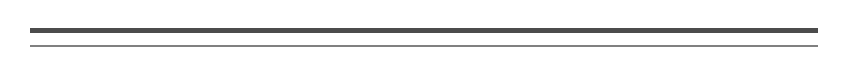
\begin{tikzpicture}
        \draw[line width=0.5pt, black!50] (0,0) -- (10,0);
        \draw[line width=2pt, black!70] (0,0.2) -- (10,0.2);
    \end{tikzpicture}
    
    \vspace{1.5cm}
    
    % Subtítulo
    {\LARGE\itshape Pauta Auxiliar 9 - Detección Bayesiana}
    
    \vspace{0.5cm}
    {\large Prof Marcos Orchard - Sebastian Espinoza.}\\
    {\large Prof Auxiliar Erik Sáez Aravena.}
    
    % Decoración con símbolo matemático de fondo
    \begin{tikzpicture}[remember picture, overlay]
        \node[opacity=0.5, rotate=0] at ([yshift=-8cm]current page.center) {
            \fontsize{200}{220}\selectfont\color{black!15}$\mathbb{E}[\Theta|X]$
        };
    \end{tikzpicture}
    
    \vfill
    
\end{center}

\newpage
%----------------------------
% =========================================
% Unidad II — Detección Bayesiana (Resumen)
% =========================================
\section{(Resumen)}

\subsection*{Modelo básico de decisión}
Sea $\{\mathcal H_i\}_{i=0}^{M-1}$ el conjunto de hipótesis, una observación $X\in\mathcal X$ con densidades condicionales $f_{X|\mathcal H_i}(x|\mathcal H_i)$, probabilidades a priori $\pi_i=P(\mathcal H_i)$ y matriz de costos $L(d_j|\mathcal H_i)$ (costo de decidir $d_j$ cuando la hipótesis verdadera es $\mathcal H_i$). El \textbf{riesgo posterior} para la acción $d_j$ dado $x$ es
\[
R(d_j|x)=\sum_{i=0}^{M-1} L(d_j|\mathcal H_i)\, P(\mathcal H_i|x).
\]
La \textbf{regla de Bayes} elige la decisión que minimiza el riesgo posterior:
\[
\delta^*(x)=\arg\min_{d_j} R(d_j|x).
\]

\subsection*{Caso binario y Regla LRT Bayesiana}
Para $M=2$ (hipótesis $\mathcal H_0$ vs. $\mathcal H_1$), con costos $L_{10}$ (falso positivo) y $L_{01}$ (falso negativo), la regla óptima se expresa como una \emph{prueba de razón de verosimilitudes} (\textit{LRT}):
\[
\Lambda(x)=\frac{f_{X|\mathcal H_1}(x)}{f_{X|\mathcal H_0}(x)} \mathop{\gtrless}_{\mathcal H_0}^{\mathcal H_1} \eta,
\qquad
\eta=\frac{L_{10}-L_{00}}{L_{01}-L_{11}}\cdot \frac{\pi_0}{\pi_1}.
\]
En el caso de costos \emph{0--1} (errores puntúan $1$ y aciertos $0$), $\eta=\pi_0/\pi_1$.

\subsection*{Regla MAP y Regla ML}
\begin{itemize}
    \item \textbf{MAP (Maximum A Posteriori):}
    \[
    \delta_{\mathrm{MAP}}(x)=\arg\max_i\, P(\mathcal H_i|x)=\arg\max_i\, \pi_i\, f_{X|\mathcal H_i}(x).
    \]
    Es óptima para costo 0--1: minimiza la probabilidad total de error.
    \item \textbf{ML (Maximum Likelihood):}
    \[
    \delta_{\mathrm{ML}}(x)=\arg\max_i\, f_{X|\mathcal H_i}(x),
    \]
    es un caso especial de MAP cuando las \emph{a priori} son uniformes.
\end{itemize}

\subsection*{Curva ROC y desempeño}
Al variar el umbral $\eta$ se obtienen pares $(P_{\mathrm{FA}},P_{\mathrm D})$ que definen la \textbf{curva ROC}. Regiones más próximas a la esquina superior izquierda indican mejores detectores. La elección del umbral se guía por costos y \emph{a priori} (óptimo Bayes) o por una cota en $P_{\mathrm{FA}}$ (criterio de Neyman--Pearson).

\subsection*{Detección Gaussiana con media conocida}
Si $X|\mathcal H_i \sim \mathcal N(\mu_i,\sigma^2)$ con varianza común, la LRT se vuelve umbral en $x$:
\[
\Lambda(x)=\exp\!\left(\frac{(\mu_1-\mu_0)}{\sigma^2}\,x - \frac{\mu_1^2-\mu_0^2}{2\sigma^2}\right) \mathop{\gtrless} \eta
\ \Longleftrightarrow\
x \mathop{\gtrless} \gamma,
\]
donde el umbral
\[
\gamma=\frac{\mu_0+\mu_1}{2} + \frac{\sigma^2}{\mu_1-\mu_0}\,\ln\eta.
\]
Con costo 0--1 y \emph{a priori} iguales, $\ln\eta=0$ y $\gamma=\tfrac{\mu_0+\mu_1}{2}$.

\subsection*{Extensión a $M$-hipótesis}
Para $M>2$:
\[
\delta^*(x)=\arg\min_{j} \sum_{i} L(d_j|\mathcal H_i)\,P(\mathcal H_i|x).
\]
Con costo 0--1:
\[
\delta_{\mathrm{MAP}}(x)=\arg\max_i\, P(\mathcal H_i|x).
\]
Cuando $f_{X|\mathcal H_i}$ y $\pi_i$ están en la familia exponencial, los \emph{suficientes} lineales permiten implementaciones por \emph{comparadores afines} (fronteras lineales/quadráticas según el caso).

\subsection*{Estimación Bayesiana (parámetros continuos)}
Sea $\Theta$ un parámetro con \emph{a priori} $p_\Theta(\theta)$ y verosimilitud $f_{X|\Theta}(x|\theta)$.
\begin{itemize}
    \item \textbf{Estimador MMSE} (pérdida cuadrática): 
    \[
    \hat\theta_{\mathrm{MMSE}}(x)=\mathbb E[\Theta|X=x].
    \]
    \item \textbf{Estimador MAP} (pérdida 0--1 asimptótica): 
    \[
    \hat\theta_{\mathrm{MAP}}(x)=\arg\max_\theta\, p_{\Theta|X}(\theta|x)\propto f_{X|\Theta}(x|\theta)\,p_\Theta(\theta).
    \]
    \item \textbf{MLE} se recupera con \emph{a priori} plana:
    \(
    \hat\theta_{\mathrm{ML}}(x)=\arg\max_\theta f_{X|\Theta}(x|\theta).
    \)
\end{itemize}
\textbf{Ejemplo (Gaussiano conjugado):} Si $X|\theta\sim \mathcal N(\theta,\sigma^2)$ y $\Theta\sim \mathcal N(\mu_0,\tau^2)$, entonces
\[
\Theta|X=x \sim \mathcal N\!\left(\frac{\tfrac{1}{\sigma^2}x+\tfrac{1}{\tau^2}\mu_0}{\tfrac{1}{\sigma^2}+\tfrac{1}{\tau^2}},\ \frac{1}{\tfrac{1}{\sigma^2}+\tfrac{1}{\tau^2}}\right),
\]
y por tanto $\hat\theta_{\mathrm{MMSE}}=\hat\theta_{\mathrm{MAP}}$ es un promedio ponderado de $x$ y $\mu_0$.

\subsection*{Riesgo Bayesiano y probabilidad de error}
El \textbf{riesgo Bayesiano} es 
\[
R_B=\mathbb E\!\left[L(\delta(X)|\mathcal H)\right]
=\sum_{i}\pi_i \int L(\delta(x)|\mathcal H_i)\, f_{X|\mathcal H_i}(x)\,dx,
\]
y bajo costo 0--1 coincide con la \emph{probabilidad total de error}. En el caso binario con LRT óptima:
\[
P_e=\pi_0\,P(\text{decidir }\mathcal H_1|\mathcal H_0)+\pi_1\,P(\text{decidir }\mathcal H_0|\mathcal H_1).
\]

%----------------------------
\newpage
\begin{questions}
\question Se pide que implemente un sistema de decisión que detecte la presencia de una señal $s_t \triangleq s(t)$. Para eso suponga que se tiene un sistema que observa $n$ muestras ruidosas de la señal $(s_k)_{k=1,...,n}$.

En concreto se distinguen dos escenarios posibles de observación.

\textbf{Presencia de señal $\Theta = 1$:}
\begin{equation}
  \begin{pmatrix} X_1 \\ X_2 \\ \vdots \\ X_n \end{pmatrix} = \begin{pmatrix} s_1 \\ s_2 \\ \vdots \\ s_n \end{pmatrix} + \begin{pmatrix} N_1 \\ N_2 \\ \vdots \\ N_n \end{pmatrix} \tag{2.87}
\end{equation}

\textbf{Ausencia de señal $\Theta = 0$:}
\begin{equation}
  \begin{pmatrix} X_1 \\ X_2 \\ \vdots \\ X_n \end{pmatrix} = \begin{pmatrix} N_1 \\ N_2 \\ \vdots \\ N_n \end{pmatrix} \tag{2.88}
\end{equation}

donde $N_1, ..., N_n$ son variables aleatorias independientes que distribuyen $\mathcal{N}(0, \sigma^2)$.

\begin{parts}
  \part Notar que dado el valor de $\Theta = \theta$, el vector $\bm{X}_1^n = (X_1, ..., X_n)$ es un vector Gaussiano. Determine su vector de media y matriz de covarianza en ambos escenarios (presencia y ausencia de señal). \textit{Indicación:} Notar que $X_1, ..., X_n$ son variables aleatorias independientes.
  
  \part Del punto anterior determine la función de log-verosimilitud
  \begin{equation*}
    L(x_1, ..., x_n|\theta) = \ln f_{X_1,...,X_n|\Theta}(x_1, ..., x_n|\theta)
  \end{equation*}
  y la solución del problema:
  \begin{equation}
    \tau_{ML}(x_1, ..., x_n) = \arg\max_{\theta \in \{0,1\}} L(x_1, ..., x_n|\theta). \tag{2.89}
  \end{equation}
  \textit{Indicación:} Se debe llegar a una expresión cerrada para $\tau_{ML}(x_1, ..., x_n)$, función de $x_1, ..., x_n$ y los parámetros conocidos del problema.
  
  \part Determine la probabilidad de error del test del punto anterior cuando $p_{\Theta}(1) = p_{\Theta}(0) = \frac{1}{2}$.
  
  \part Determine que pasa con la probabilidad de error del test óptimo en (2.89), si la potencia de la señal dada por $||s||^2 = \sum_{i=1}^{n} s_i^2$ tiende a infinito, es decir,
  \begin{equation*}
    \lim_{n \to \infty} ||s||^2 = \infty
  \end{equation*}
\end{parts}
    
%----------------------------
\newpage
\begin{solution}
\subsection*{Resolución 1.1}

Analizamos el vector aleatorio $\bm{X}_1^n = (X_1, ..., X_n)^T$ bajo ambas hipótesis.
\begin{itemize}
  \item  \textbf{Caso $\Theta = 1$ (Presencia de señal):}

De la ecuación (2.87), tenemos que $X_i = s_i + N_i$ para $i = 1, ..., n$. Como los $N_i$ son independientes con $N_i \sim \mathcal{N}(0, \sigma^2)$ y la señal $s_i$ es determinista:

Primero calculamos el vector de media y la matriz de covarianza. Para lo primero tenemos que:
\begin{equation*}
  \mathbb{E}[X_i|\Theta = 1] = \mathbb{E}[s_i + N_i] = s_i + \mathbb{E}[N_i] = s_i
\end{equation*}
Por lo tanto:
\begin{equation*}
  \bm{\mu}_1 = \mathbb{E}[\bm{X}_1^n|\Theta = 1] = \begin{pmatrix} s_1 \\ s_2 \\ \vdots \\ s_n \end{pmatrix} = \bm{s}
\end{equation*}


Ahora debemos caracterizar cómo varían las observaciones alrededor de su media. Para un vector aleatorio $\bm{X} = (X_1, ..., X_n)^T$, la matriz de covarianza $\bm{\Sigma}$ captura tanto:
\begin{itemize}
  \item La variabilidad de cada variable individual (elementos diagonales)
  \item La relación lineal entre pares de variables (elementos fuera de la diagonal)
\end{itemize}
La matriz de covarianza se define como:
\begin{equation*}
  \bm{\Sigma} = \mathbb{E}[(\bm{X} - \bm{\mu})(\bm{X} - \bm{\mu})^T]
\end{equation*}

donde cada elemento $(i,j)$ de esta matriz es:
\begin{equation*}
  \Sigma_{ij} = \mathbb{E}[(X_i - \mu_i)(X_j - \mu_j)] = \text{Cov}(X_i, X_j)
\end{equation*}

Esta matriz es fundamental en el análisis de vectores Gaussianos porque especifica completamente la estructura de correlación entre las componentes del vector.

Luego, para la matriz de covarianza en nuestro problema, recordemos que como las variables $N_i$ son independientes, entonces:
\begin{equation*}
  \text{Cov}(X_i, X_j|\Theta = 1) = \text{Cov}(s_i + N_i, s_j + N_j) = \text{Cov}(N_i, N_j) = \begin{cases}
    \sigma^2 & \text{si } i = j \\
    0 & \text{si } i \neq j
  \end{cases}
\end{equation*}

La matriz de covarianza $\bm{\Sigma}_1$ es una matriz de $n \times n$ donde el elemento $(i,j)$ es $\text{Cov}(X_i, X_j|\Theta = 1)$. Explícitamente, esta matriz tiene la forma:
\begin{equation*}
  \bm{\Sigma}_1 = \begin{pmatrix}
    \text{Cov}(X_1, X_1) & \text{Cov}(X_1, X_2) & \cdots & \text{Cov}(X_1, X_n) \\
    \text{Cov}(X_2, X_1) & \text{Cov}(X_2, X_2) & \cdots & \text{Cov}(X_2, X_n) \\
    \vdots & \vdots & \ddots & \vdots \\
    \text{Cov}(X_n, X_1) & \text{Cov}(X_n, X_2) & \cdots & \text{Cov}(X_n, X_n)
  \end{pmatrix}
\end{equation*}

Sustituyendo los valores de las covarianzas (las varianzas $\sigma^2$ en la diagonal y ceros fuera de ella):
\begin{equation*}
  \bm{\Sigma}_1 = \begin{pmatrix}
    \sigma^2 & 0 & \cdots & 0 \\
    0 & \sigma^2 & \cdots & 0 \\
    \vdots & \vdots & \ddots & \vdots \\
    0 & 0 & \cdots & \sigma^2
  \end{pmatrix} = \sigma^2 \begin{pmatrix}
    1 & 0 & \cdots & 0 \\
    0 & 1 & \cdots & 0 \\
    \vdots & \vdots & \ddots & \vdots \\
    0 & 0 & \cdots & 1
  \end{pmatrix} = \sigma^2 \bm{I}_n
\end{equation*}

donde $\bm{I}_n$ es la matriz identidad de $n \times n$. Esta estructura diagonal refleja la independencia entre las observaciones $X_i$, ya que todas tienen la misma varianza $\sigma^2$ y covarianza cero entre ellas.

\item \textbf{Caso $\Theta = 0$ (Ausencia de señal):}

De la ecuación, tenemos que $X_i = N_i$ para $i = 1, ..., n$, por lo que analogamente tenemos que:
\begin{equation*}
  \bm{\mu}_0 = \mathbb{E}[\bm{X}_1^n|\Theta = 0] = \begin{pmatrix} 0 \\ 0 \\ \vdots \\ 0 \end{pmatrix} = \bm{0}
\end{equation*}

y por otro lado:
\begin{equation*}
  \bm{\Sigma}_0 = \sigma^2 \bm{I}_n
\end{equation*}
\end{itemize}
\subsection*{Resolución 1.2}

La regla de Máxima Verosimilitud (ML, por sus siglas en inglés \textit{Maximum Likelihood}) es un caso particular de la regla MAP cuando las hipótesis son equiprobables o no se tienen priors informativos. Como $\Sigma_0 = \Sigma_1$ y no se especifican costos ni priors distintos, con $p_{\Theta}(0) = p_{\Theta}(1)$, la regla MAP coincide con ML.

Matemáticamente, la regla ML decide la hipótesis $\theta^*$ que maximiza la función de verosimilitud:
\begin{equation*}
  \theta^* = \arg\max_{\theta \in \Theta} f_{X|\Theta}(x|\theta)
\end{equation*}

Equivalentemente, podemos maximizar la log-verosimilitud (que es más conveniente computacionalmente):
\begin{equation*}
  \theta^* = \arg\max_{\theta \in \Theta} L(x|\theta) = \arg\max_{\theta \in \Theta} \ln f_{X|\Theta}(x|\theta)
\end{equation*}
Sabemos que la función de densidad para un vector Gaussiano multivariado es:
\begin{equation*}
  f_{\bm{X}_1^n|\Theta}(\bm{x}|\theta) = \frac{1}{(2\pi)^{n/2}|\bm{\Sigma}_\theta|^{1/2}} \exp\left(-\frac{1}{2}(\bm{x} - \bm{\mu}_\theta)^T \bm{\Sigma}_\theta^{-1} (\bm{x} - \bm{\mu}_\theta)\right)
\end{equation*}

Luego al aplicar el logaritmo, obtenemos la log-verosimilitud:
\begin{align*}
  L(\bm{x}|\theta) &= \ln f_{\bm{X}_1^n|\Theta}(\bm{x}|\theta) \\
  &= -\frac{n}{2}\ln(2\pi) - \frac{1}{2}\ln|\bm{\Sigma}_\theta| - \frac{1}{2}(\bm{x} - \bm{\mu}_\theta)^T \bm{\Sigma}_\theta^{-1} (\bm{x} - \bm{\mu}_\theta)
\end{align*}

Para $\theta = 1$:
\begin{align*}
  L(\bm{x}|1) &= -\frac{n}{2}\ln(2\pi) - \frac{n}{2}\ln(\sigma^2) - \frac{1}{2\sigma^2}\sum_{i=1}^{n}(x_i - s_i)^2 \\
  &= -\frac{n}{2}\ln(2\pi\sigma^2) - \frac{1}{2\sigma^2}\sum_{i=1}^{n}(x_i - s_i)^2
\end{align*}

Para $\theta = 0$:
\begin{align*}
  L(\bm{x}|0) &= -\frac{n}{2}\ln(2\pi\sigma^2) - \frac{1}{2\sigma^2}\sum_{i=1}^{n}x_i^2
\end{align*}

Para determinar $\tau_{ML}(\bm{x})$, comparamos las log-verosimilitudes:
\begin{align*}
  \tau_{ML}(\bm{x}) = 1 &\iff L(\bm{x}|1) > L(\bm{x}|0) \\
  &\iff -\frac{1}{2\sigma^2}\sum_{i=1}^{n}(x_i - s_i)^2 > -\frac{1}{2\sigma^2}\sum_{i=1}^{n}x_i^2 \\
  &\iff \sum_{i=1}^{n}(x_i - s_i)^2 < \sum_{i=1}^{n}x_i^2 \\
  &\iff \sum_{i=1}^{n}(x_i^2 - 2x_is_i + s_i^2) < \sum_{i=1}^{n}x_i^2 \\
  &\iff -2\sum_{i=1}^{n}x_is_i + \sum_{i=1}^{n}s_i^2 < 0 \\
  &\iff \sum_{i=1}^{n}x_is_i > \frac{1}{2}\sum_{i=1}^{n}s_i^2 = \frac{||s||^2}{2}
\end{align*}

Por lo que se llega a la siguiente regla de decisión:
\begin{equation*}
  \tau_{ML}(x_1, ..., x_n) = \begin{cases}
    1 & \text{si } T = \sum_{i=1}^{n}x_is_i > \frac{||s||^2}{2} \\
    0 & \text{en caso contrario}
  \end{cases}
\end{equation*}

donde el umbral $\frac{||s||^2}{2}$ corresponde al punto medio entre las medias de $T$ bajo ambas hipótesis.

\subsection*{Resolución 1.3}

Con $p_{\Theta}(1) = p_{\Theta}(0) = \frac{1}{2}$, la probabilidad de error es:
\begin{align*}
  P_e &= P(\tau_{ML} = 0, \Theta = 1) + P(\tau_{ML} = 1, \Theta = 0) \\
  &= P(\Theta = 1)P(\tau_{ML} = 0|\Theta = 1) + P(\Theta = 0)P(\tau_{ML} = 1|\Theta = 0) \\
  &= \frac{1}{2}P\left(\sum_{i=1}^{n}X_is_i \leq \frac{||s||^2}{2}\bigg|\Theta = 1\right) + \frac{1}{2}P\left(\sum_{i=1}^{n}X_is_i > \frac{||s||^2}{2}\bigg|\Theta = 0\right)
\end{align*}

Analizamos la distribución de $\sum_{i=1}^{n}X_is_i$ bajo cada hipótesis.

\textbf{Bajo $\Theta = 1$:} Como $X_i = s_i + N_i$, tenemos:
\begin{align*}
  \sum_{i=1}^{n}X_is_i &= \sum_{i=1}^{n}(s_i + N_i)s_i = \sum_{i=1}^{n}s_i^2 + \sum_{i=1}^{n}N_is_i = ||s||^2 + \sum_{i=1}^{n}N_is_i
\end{align*}
Como $N_i \sim \mathcal{N}(0, \sigma^2)$ son independientes, la suma $\sum_{i=1}^{n}N_is_i$ es Gaussiana con media cero y varianza $\sigma^2\sum_{i=1}^{n}s_i^2 = \sigma^2||s||^2$. Por lo tanto:
\begin{equation*}
  \sum_{i=1}^{n}X_is_i\bigg|\Theta = 1 \sim \mathcal{N}(||s||^2, \sigma^2||s||^2)
\end{equation*}

\textbf{Bajo $\Theta = 0$:} Como $X_i = N_i$, entonces:
\begin{equation*}
  \sum_{i=1}^{n}X_is_i\bigg|\Theta = 0 = \sum_{i=1}^{n}N_is_i \sim \mathcal{N}(0, \sigma^2||s||^2)
\end{equation*}

Ahora calculamos las probabilidades. Para $\Theta = 1$, estandarizamos:
\begin{align*}
  P\left(\sum_{i=1}^{n}X_is_i \leq \frac{||s||^2}{2}\bigg|\Theta = 1\right) &= P\left(\frac{\sum_{i=1}^{n}X_is_i - ||s||^2}{\sigma||s||} \leq \frac{-||s||^2/2}{\sigma||s||}\bigg|\Theta = 1\right) \\
  &= P\left(Z \leq -\frac{||s||}{2\sigma}\right) = Q\left(\frac{||s||}{2\sigma}\right)
\end{align*}
donde $Z \sim \mathcal{N}(0, 1)$ y $Q(x) = P(Z > x)$ es la función Q.

Para $\Theta = 0$:
\begin{align*}
  P\left(\sum_{i=1}^{n}X_is_i > \frac{||s||^2}{2}\bigg|\Theta = 0\right) &= P\left(\frac{\sum_{i=1}^{n}X_is_i}{\sigma||s||} > \frac{||s||^2/2}{\sigma||s||}\bigg|\Theta = 0\right) \\
  &= P\left(Z > \frac{||s||}{2\sigma}\right) = Q\left(\frac{||s||}{2\sigma}\right)
\end{align*}

Por simetría, ambos términos son iguales, por lo tanto:
\begin{equation*}
  P_e = \frac{1}{2}Q\left(\frac{||s||}{2\sigma}\right) + \frac{1}{2}Q\left(\frac{||s||}{2\sigma}\right) = Q\left(\frac{||s||}{2\sigma}\right)
\end{equation*}

\subsection*{Resolución 1.4}

Del punto anterior, tenemos que la probabilidad de error es:
\begin{equation*}
  P_e = Q\left(\frac{||s||}{2\sigma}\right)
\end{equation*}

Cuando $||s||^2 \to \infty$, entonces $||s|| \to \infty$, y por lo tanto:
\begin{equation*}
  \lim_{||s|| \to \infty} P_e = \lim_{||s|| \to \infty} Q\left(\frac{||s||}{2\sigma}\right) = Q(\infty) = 0
\end{equation*}

Podemos entenerlo como cuando la potencia de la señal tiende a infinito, el test de máxima verosimilitud puede distinguir perfectamente entre presencia y ausencia de señal, ya que la probabilidad de error tiende a cero. Esto tiene sentido físicamente: una señal con potencia infinita es fácilmente distinguible del ruido, sin importar cuán grande sea la varianza del ruido.
\end{solution}

%----------------------------
\newpage
\question El estudiante Juanito fue a una degustación a ciegas en el Paseo Eléctrico. Lamentablemente Juanito estaba muy congestionado por lo que le costaba identificar los sabores y además por ser una degustación a ciegas no sabía cuál bebida estaba tomando. Se sabe que este local durante la degustación ofreció 3 tipos de bebidas: vino, pisco y baltica, además, la frecuencia con la cuál salía cada bebida del bar era del 50\%, 20\% y 30\% respectivamente. Las bebidas pueden gustarle o no gustarle a Juanito y, por experiencia, él sabe que si la bebida es vino le gusta el 40\% de las veces, si es pisco le gusta el 20\% de las veces y si es baltica le gusta el 70\% de las veces. Juanito probó la bebida recibida y le gustó. El objetivo de esta pregunta es que usted ayude a Juanito a detectar cuál fue la bebida que tomó. Para esto siga los siguientes pasos:

\begin{parts}
  \part Plantee un espacio de observación y un espacio de decisión adecuado, indique la distribución de la variable aleatoria $\Theta$ asociado al espacio de decisión (distribución a priori) y las densidades y/o probabilidades de masa condicionales de $X$ dado $\Theta = \theta$.
  
  \part Suponga que la función de costo del problema Bayesiano es la función $L_{0,1}$, es decir,
  \begin{equation}
    L_{0,1}(x, y) = \begin{cases}
      1 & \text{si } x \neq y \\
      0 & \text{si } x = y.
    \end{cases} \tag{2.90}
  \end{equation}
  Plantee la regla óptima de decisión y a partir de esto decida cuál fue la bebida que tomó.
\end{parts}
  
\begin{solution}
\subsection*{Resolución 2.1}

Para plantear el problema de decisión Bayesiana, debemos identificar los espacios y distribuciones involucradas.

El espacio de decisión corresponde al tipo de bebida que Juanito debe identificar:
\begin{equation*}
  \Theta = \{\text{Vino}, \text{Pisco}, \text{Baltica}\} = \{V, P, B\}
\end{equation*}


La distribución a priori $p_\Theta(\theta)$ corresponde a la frecuencia con que sale cada bebida del bar:
\begin{align*}
  p_\Theta(V) &= 0.50 \\
  p_\Theta(P) &= 0.20 \\
  p_\Theta(B) &= 0.30
\end{align*}


El espacio de observación corresponde a si la bebida le gustó o no a Juanito:
\begin{equation*}
  \mathcal{X} = \{\text{Gusta}, \text{No Gusta}\} = \{1, 0\}
\end{equation*}

Las probabilidades de masa condicionales $P_{X|\Theta}(x|\theta)$ representan la probabilidad de que a Juanito le guste la bebida dado el tipo de bebida:

Para $X = 1$ (le gusta):
\begin{align*}
  P_{X|\Theta}(1|V) &= 0.40 \\
  P_{X|\Theta}(1|P) &= 0.20 \\
  P_{X|\Theta}(1|B) &= 0.70
\end{align*}

Para $X = 0$ (no le gusta):
\begin{align*}
  P_{X|\Theta}(0|V) &= 1 - 0.40 = 0.60 \\
  P_{X|\Theta}(0|P) &= 1 - 0.20 = 0.80 \\
  P_{X|\Theta}(0|B) &= 1 - 0.70 = 0.30
\end{align*}

\subsection*{Resolución 2.2}

Con la función de costo $L_{0,1}$ dada en (2.90), el riesgo Bayesiano para una regla de decisión $\delta(x)$ es:
\begin{align*}
  r(\delta) &= \mathbb{E}_{X,\Theta}[L_{0,1}(\Theta, \delta(X))] \\
  &= P(\Theta \neq \delta(X)) \\
  &= P(\text{error})
\end{align*}

Es decir, minimizar el riesgo equivale a minimizar la probabilidad de error. La regla de decisión óptima es el estimador MAP:
\begin{equation*}
  \delta^*(x) = \arg\max_{\theta \in \{V, P, B\}} p_{\Theta|X}(\theta|x)
\end{equation*}

Usando el teorema de Bayes:
\begin{equation*}
  p_{\Theta|X}(\theta|x) = \frac{P_{X|\Theta}(x|\theta) \cdot p_\Theta(\theta)}{p_X(x)}
\end{equation*}

Como $p_X(x)$ es constante para todas las hipótesis, podemos comparar directamente:
\begin{equation*}
  \delta^*(x) = \arg\max_{\theta \in \{V, P, B\}} P_{X|\Theta}(x|\theta) \cdot p_\Theta(\theta)
\end{equation*}

Juanito observó que le gustó la bebida, es decir, $X = 1$. Calculamos las probabilidades a posteriori (sin normalizar):

\begin{align*}
  P_{X|\Theta}(1|V) \cdot p_\Theta(V) &= 0.40 \times 0.50 = 0.20 \\
  P_{X|\Theta}(1|P) \cdot p_\Theta(P) &= 0.20 \times 0.20 = 0.04 \\
  P_{X|\Theta}(1|B) \cdot p_\Theta(B) &= 0.70 \times 0.30 = 0.21
\end{align*}

Comparando los valores:
\begin{equation*}
  \max\{0.20, 0.04, 0.21\} = 0.21
\end{equation*}

La regla de decisión óptima indica que Juanito tomó \textbf{baltica}, ya que es la hipótesis con mayor probabilidad a posteriori dado que le gustó la bebida.

Primero calculamos $p_X(1)$:
\begin{equation*}
  p_X(1) = 0.20 + 0.04 + 0.21 = 0.45
\end{equation*}

Las probabilidades a posteriori normalizadas son:
\begin{align*}
  p_{\Theta|X}(V|1) &= \frac{0.20}{0.45} = 0.444 \approx 44.4\% \\
  p_{\Theta|X}(P|1) &= \frac{0.04}{0.45} = 0.089 \approx 8.9\% \\
  p_{\Theta|X}(B|1) &= \frac{0.21}{0.45} = 0.467 \approx 46.7\%
\end{align*}

La baltica tiene la mayor probabilidad a posteriori (46.7\%), confirmando nuestra decisión óptima.

\end{solution}

%----------------------------
\newpage
\question Considere un problema de detección Bayesiano con un espacio de observación $\mathbb{X}$ arbitrario tal que $\Theta = \{0, 1\}$, es decir, un problema de decisión binario. Además considere la función de costo $L_{0,1}$.

\begin{parts}
  \part Demuestre que en este caso la regla óptima puede escribirse como:
  \begin{equation}
    r^*(x) = \begin{cases}
      1 & \text{si } \eta(x) > 1/2 \\
      0 & \text{si } \eta(x) < 1/2 \\
      I & \text{si } \eta(x) = 1/2
    \end{cases} \tag{2.91}
  \end{equation}
  donde $\eta(x) = P_{\Theta|X}(\Theta = 1|X = x)$ e $I$ indica indiferencia, es decir, 0 o 1.
  
  \part Demuestre que para cualquier otra regla de decisión $\pi : \mathbb{X} \to \{0, 1\}$ se tiene que:
  \begin{equation*}
    P_{X,\Theta}(r^*(X) \neq \Theta) \leq P_{X,\Theta}(\pi(X) \neq \Theta).
  \end{equation*}
  Es decir, la regla $r^*$ es aquella que minimiza la probabilidad de error. Para esto use el hecho que, dado $x \in \mathbb{X}$ y una regla $\pi : \mathbb{X} \to \{0, 1\}$ arbitraria entonces:
  \begin{equation}
    P_{\Theta|X}(\pi(X) \neq \Theta|X = x) = 1 - \left[\mathbf{1}_{\pi(x)=1}(x) \cdot \eta(x) + \mathbf{1}_{\pi(x)=0}(x) \cdot (1 - \eta(x))\right], \tag{2.92}
  \end{equation}
  donde $\mathbf{1}_B(x)$ corresponde a la indicatriz, es decir, vale 1 si $x \in B$ y 0 en caso contrario.
\end{parts}
    
\begin{solution}
\subsection*{Resolución 3.1}

Para encontrar la regla de decisión óptima bajo la función de costo $L_{0,1}$, debemos minimizar el riesgo Bayesiano.

Con la función de costo $L_{0,1}$, tenemos:
\begin{equation*}
  L_{0,1}(\theta, \delta) = \begin{cases}
    0 & \text{si } \theta = \delta \\
    1 & \text{si } \theta \neq \delta
  \end{cases}
\end{equation*}

El riesgo Bayesiano condicional para una decisión $\delta$ dado $X = x$ es:
\begin{align*}
  r(\delta|x) &= \mathbb{E}_{\Theta|X}[L_{0,1}(\Theta, \delta)|X = x] \\
  &= \sum_{\theta \in \{0,1\}} L_{0,1}(\theta, \delta) \cdot P_{\Theta|X}(\theta|x)
\end{align*}

Para $\delta = 1$:
\begin{align*}
  r(1|x) &= L_{0,1}(0, 1) \cdot P_{\Theta|X}(0|x) + L_{0,1}(1, 1) \cdot P_{\Theta|X}(1|x) \\
  &= 1 \cdot P_{\Theta|X}(0|x) + 0 \cdot P_{\Theta|X}(1|x) \\
  &= P_{\Theta|X}(0|x) = 1 - \eta(x)
\end{align*}

Para $\delta = 0$:
\begin{align*}
  r(0|x) &= L_{0,1}(0, 0) \cdot P_{\Theta|X}(0|x) + L_{0,1}(1, 0) \cdot P_{\Theta|X}(1|x) \\
  &= 0 \cdot P_{\Theta|X}(0|x) + 1 \cdot P_{\Theta|X}(1|x) \\
  &= P_{\Theta|X}(1|x) = \eta(x)
\end{align*}

La regla óptima minimiza el riesgo condicional para cada $x$:
\begin{equation*}
  r^*(x) = \arg\min_{\delta \in \{0,1\}} r(\delta|x)
\end{equation*}

Comparando los riesgos:
\begin{align*}
  r^*(x) = 1 &\iff r(1|x) < r(0|x) \\
  &\iff 1 - \eta(x) < \eta(x) \\
  &\iff 1 < 2\eta(x) \\
  &\iff \eta(x) > \frac{1}{2}
\end{align*}

Similarmente:
\begin{align*}
  r^*(x) = 0 &\iff \eta(x) < \frac{1}{2}
\end{align*}

Cuando $\eta(x) = 1/2$, ambos riesgos son iguales ($r(0|x) = r(1|x) = 1/2$), por lo que hay indiferencia.

Por lo tanto, la regla óptima es:
\begin{equation*}
  r^*(x) = \begin{cases}
    1 & \text{si } \eta(x) > 1/2 \\
    0 & \text{si } \eta(x) < 1/2 \\
    I & \text{si } \eta(x) = 1/2
  \end{cases}
\end{equation*}

\subsection*{Resolución 3.2}

Para demostrar que $r^*$ minimiza la probabilidad de error, usamos la expresión (2.92) y el teorema de la probabilidad total. La probabilidad de error para una regla $\pi$ es:
\begin{align*}
  P_{X,\Theta}(\pi(X) \neq \Theta) &= \mathbb{E}_X[P_{\Theta|X}(\pi(X) \neq \Theta|X)] \\
  &= \int_{\mathbb{X}} P_{\Theta|X}(\pi(X) \neq \Theta|X = x) \, dP_X(x)
\end{align*}

Usando la ecuación (2.92):
\begin{equation*}
  P_{\Theta|X}(\pi(X) \neq \Theta|X = x) = 1 - \left[\mathbf{1}_{\pi(x)=1}(x) \cdot \eta(x) + \mathbf{1}_{\pi(x)=0}(x) \cdot (1 - \eta(x))\right]
\end{equation*}

Notemos que para cualquier $x$, se cumple que $\mathbf{1}_{\pi(x)=1}(x) + \mathbf{1}_{\pi(x)=0}(x) = 1$, ya que $\pi(x) \in \{0, 1\}$.

Podemos reescribir:
\begin{align*}
  &\mathbf{1}_{\pi(x)=1}(x) \cdot \eta(x) + \mathbf{1}_{\pi(x)=0}(x) \cdot (1 - \eta(x)) \\
  &= \mathbf{1}_{\pi(x)=1}(x) \cdot \eta(x) + [1 - \mathbf{1}_{\pi(x)=1}(x)] \cdot (1 - \eta(x)) \\
  &= \mathbf{1}_{\pi(x)=1}(x) \cdot \eta(x) + (1 - \eta(x)) - \mathbf{1}_{\pi(x)=1}(x) \cdot (1 - \eta(x)) \\
  &= (1 - \eta(x)) + \mathbf{1}_{\pi(x)=1}(x) \cdot [2\eta(x) - 1]
\end{align*}

Por lo tanto:
\begin{equation*}
  P_{\Theta|X}(\pi(X) \neq \Theta|X = x) = \eta(x) - \mathbf{1}_{\pi(x)=1}(x) \cdot [2\eta(x) - 1]
\end{equation*}

Para minimizar esta expresión dado $x$, debemos elegir $\mathbf{1}_{\pi(x)=1}(x)$ óptimamente:

\begin{itemize}
  \item Si $2\eta(x) - 1 > 0$ (es decir, $\eta(x) > 1/2$): elegimos $\mathbf{1}_{\pi(x)=1}(x) = 1$, o sea $\pi(x) = 1$.
  \item Si $2\eta(x) - 1 < 0$ (es decir, $\eta(x) < 1/2$): elegimos $\mathbf{1}_{\pi(x)=1}(x) = 0$, o sea $\pi(x) = 0$.
  \item Si $2\eta(x) - 1 = 0$ (es decir, $\eta(x) = 1/2$): cualquier decisión da el mismo resultado.
\end{itemize}

Esta es exactamente la regla $r^*(x)$ definida en (2.91).

Como $r^*$ minimiza $P_{\Theta|X}(\pi(X) \neq \Theta|X = x)$ para cada $x \in \mathbb{X}$, también minimiza la probabilidad de error total:
\begin{equation*}
  P_{X,\Theta}(r^*(X) \neq \Theta) = \int_{\mathbb{X}} \min_{\delta \in \{0,1\}} P_{\Theta|X}(\delta \neq \Theta|X = x) \, dP_X(x)
\end{equation*}

Por lo tanto, para cualquier otra regla $\pi$:
\begin{equation*}
  P_{X,\Theta}(r^*(X) \neq \Theta) \leq P_{X,\Theta}(\pi(X) \neq \Theta)
\end{equation*}

Esto demuestra que $r^*$ es la regla óptima que minimiza la probabilidad de error.

\end{solution}

%----------------------------
\newpage
\question Considere un cuerpo radiactivo que emite $\theta$ partículas, con $\theta \in \mathbb{N}$. Para detectar las partículas emitidas, se cuenta con un detector imperfecto, el cual detecta cada partícula emitida de forma independiente. Para modelar el proceso de detección, consideremos la variable aleatoria $B_i$ que toma el valor 1 si la partícula $i$-ésima fue detectada y 0 si no, donde $B_i$ distribuye Bernoulli de parámetro $p$ ($P_{B_i}(B_i = 1) = p$).

Finalmente, la variable de observación $X$ es el número de partículas totales detectadas dada por
\begin{equation*}
  X = \sum_{i=1}^{\theta} B_i \in \{0, \cdots, \theta\}
\end{equation*}
Notar que dados $p$ y $\theta$ conocidos, $X$ distribuye binomial de parámetros $p$ y $\theta$, es decir:
\begin{equation*}
  P_X(X = k|p, \theta) = \binom{\theta}{k} p^k (1-p)^{\theta-k}
\end{equation*}

Considere el problema de estimar la cantidad de partículas emitidas $\theta$ asumiendo conocido $p$, pero en un contexto Bayesiano, donde la cantidad de partículas emitidas distribuye Poisson de parámetro $\lambda$ conocido, es decir:
\begin{equation*}
  p_{\Theta}(\theta) = \frac{\lambda^{\theta}}{\theta!} e^{-\lambda}, \quad \forall \theta \in \{0, 1, 2, \cdots\}
\end{equation*}

Luego, se busca el estimador que minimice el error cuadrático medio $\phi_{MMSE}(X)$, dada una observación de $X$. Para ello, siga los siguientes pasos:

\begin{parts}
  \part Determine la probabilidad conjunta $P_{X,\Theta}(X = k, \Theta = \theta)$ y con ello muestre que la variable aleatoria $X$ (número de partículas detectadas) distribuye Poisson de parámetro $\lambda p$, es decir:
  \begin{equation*}
    p_X(k) = \frac{(\lambda p)^k}{k!} e^{-\lambda p}, \quad \forall k \in \{0, 1, 2, \cdots\}
  \end{equation*}
  
  \part Muestre que:
  \begin{equation*}
    P_{\Theta|X}(\Theta = \theta|X = k) = \frac{(\lambda(1-p))^{\theta-k}}{(\theta - k)!} e^{-\lambda(1-p)}, \quad \text{si } \theta \geq k
  \end{equation*}
  y
  \begin{equation*}
    P_{\Theta|X}(\theta|k) = 0 \quad \text{si } \theta < k
  \end{equation*}
  y con ello obtenga $\pi_{MMSE}(X)$. Comente sobre los regímenes $p \approx 1$ y $p \approx 0$.
\end{parts}

%----------------------------
\newpage
\begin{solution}
\subsection*{Resolución 4.1}

Para encontrar la distribución marginal de $X$, primero calculamos la distribución conjunta y luego marginalizamos sobre $\Theta$.
\begin{align*}
  P_{X,\Theta}(X = k, \Theta = \theta) &= P_{X|\Theta}(X = k|\Theta = \theta) \cdot P_{\Theta}(\theta) \\
  &= \binom{\theta}{k} p^k (1-p)^{\theta-k} \cdot \frac{\lambda^{\theta}}{\theta!} e^{-\lambda}
\end{align*}

Para $\theta \geq k$:
\begin{align*}
  P_{X,\Theta}(k, \theta) &= \frac{\theta!}{k!(\theta-k)!} p^k (1-p)^{\theta-k} \cdot \frac{\lambda^{\theta}}{\theta!} e^{-\lambda} \\
  &= \frac{p^k (1-p)^{\theta-k} \lambda^{\theta}}{k!(\theta-k)!} e^{-\lambda}
\end{align*}

Para $\theta < k$: $P_{X,\Theta}(k, \theta) = 0$ (no se pueden detectar más partículas de las emitidas).


\begin{align*}
  p_X(k) &= \sum_{\theta=0}^{\infty} P_{X,\Theta}(k, \theta) \\
  &= \sum_{\theta=k}^{\infty} \frac{p^k (1-p)^{\theta-k} \lambda^{\theta}}{k!(\theta-k)!} e^{-\lambda} \\
  &= \frac{p^k e^{-\lambda}}{k!} \sum_{\theta=k}^{\infty} \frac{(1-p)^{\theta-k} \lambda^{\theta}}{(\theta-k)!}
\end{align*}

Hacemos el cambio de variable $m = \theta - k$:
\begin{align*}
  p_X(k) &= \frac{p^k e^{-\lambda}}{k!} \sum_{m=0}^{\infty} \frac{(1-p)^m \lambda^{m+k}}{m!} \\
  &= \frac{p^k \lambda^k e^{-\lambda}}{k!} \sum_{m=0}^{\infty} \frac{[\lambda(1-p)]^m}{m!} \\
  &= \frac{(p\lambda)^k e^{-\lambda}}{k!} \cdot e^{\lambda(1-p)} \\
  &= \frac{(\lambda p)^k}{k!} e^{-\lambda + \lambda(1-p)} \\
  &= \frac{(\lambda p)^k}{k!} e^{-\lambda p}
\end{align*}

Por lo tanto, $X \sim \text{Poisson}(\lambda p)$.

\subsection*{Resolución 4.2}


Usando el teorema de Bayes:
\begin{equation*}
  P_{\Theta|X}(\theta|k) = \frac{P_{X,\Theta}(k, \theta)}{p_X(k)}
\end{equation*}

Para $\theta \geq k$:
\begin{align*}
  P_{\Theta|X}(\theta|k) &= \frac{\frac{p^k (1-p)^{\theta-k} \lambda^{\theta}}{k!(\theta-k)!} e^{-\lambda}}{\frac{(\lambda p)^k}{k!} e^{-\lambda p}} \\
  &= \frac{p^k (1-p)^{\theta-k} \lambda^{\theta} e^{-\lambda}}{(\theta-k)!} \cdot \frac{k!}{(\lambda p)^k e^{-\lambda p}} \\
  &= \frac{(1-p)^{\theta-k} \lambda^{\theta} e^{-\lambda}}{(\theta-k)!} \cdot \frac{1}{\lambda^k e^{-\lambda p}} \\
  &= \frac{\lambda^{\theta-k} (1-p)^{\theta-k}}{(\theta-k)!} e^{-\lambda + \lambda p} \\
  &= \frac{[\lambda(1-p)]^{\theta-k}}{(\theta-k)!} e^{-\lambda(1-p)}
\end{align*}

Para $\theta < k$: $P_{\Theta|X}(\theta|k) = 0$.

Observamos que dado $X = k$, la variable $\Theta$ tiene una distribución Poisson desplazada: $\Theta - k \sim \text{Poisson}(\lambda(1-p))$.

El estimador MMSE es la esperanza condicional:
\begin{align*}
  \pi_{MMSE}(k) &= \mathbb{E}[\Theta|X = k] \\
  &= \sum_{\theta=k}^{\infty} \theta \cdot P_{\Theta|X}(\theta|k) \\
  &= \sum_{\theta=k}^{\infty} \theta \cdot \frac{[\lambda(1-p)]^{\theta-k}}{(\theta-k)!} e^{-\lambda(1-p)}
\end{align*}

Usando el cambio de variable $m = \theta - k$:
\begin{align*}
  \pi_{MMSE}(k) &= \sum_{m=0}^{\infty} (m + k) \cdot \frac{[\lambda(1-p)]^m}{m!} e^{-\lambda(1-p)} \\
  &= k \sum_{m=0}^{\infty} \frac{[\lambda(1-p)]^m}{m!} e^{-\lambda(1-p)} + \sum_{m=0}^{\infty} m \cdot \frac{[\lambda(1-p)]^m}{m!} e^{-\lambda(1-p)} \\
  &= k \cdot 1 + \lambda(1-p) \\
  &= k + \lambda(1-p)
\end{align*}

Por lo tanto:
\begin{equation*}
  \boxed{\pi_{MMSE}(X) = X + \lambda(1-p)}
\end{equation*}

\textbf{Análisis de regímenes:}

\begin{itemize}
  \item \textbf{Régimen $p \approx 1$ (detector casi perfecto):} 
  \begin{equation*}
    \pi_{MMSE}(X) \approx X + \lambda(1-1) = X
  \end{equation*}
  El estimador es aproximadamente igual al número de partículas detectadas, lo cual tiene sentido ya que el detector detecta casi todas las partículas emitidas.
  
  \item \textbf{Régimen $p \approx 0$ (detector muy malo):}
  \begin{equation*}
    \pi_{MMSE}(X) \approx X + \lambda(1-0) = X + \lambda
  \end{equation*}
  El estimador se sesga fuertemente hacia el prior $\lambda$. Como el detector detecta muy pocas partículas, la observación $X$ es poco informativa y el estimador se apoya más en la información a priori. El término $X$ es pequeño (pocas detecciones) y el término $\lambda$ domina, estimando cerca del valor esperado a priori.
\end{itemize}

\end{solution}
\end{questions}
\end{document}